\thispagestyle{empty}

\newgeometry{tmargin=2cm, bmargin=2cm, lmargin=2cm, rmargin=2cm}

\begin{figure*}[H] \begin{center}
    \centerline{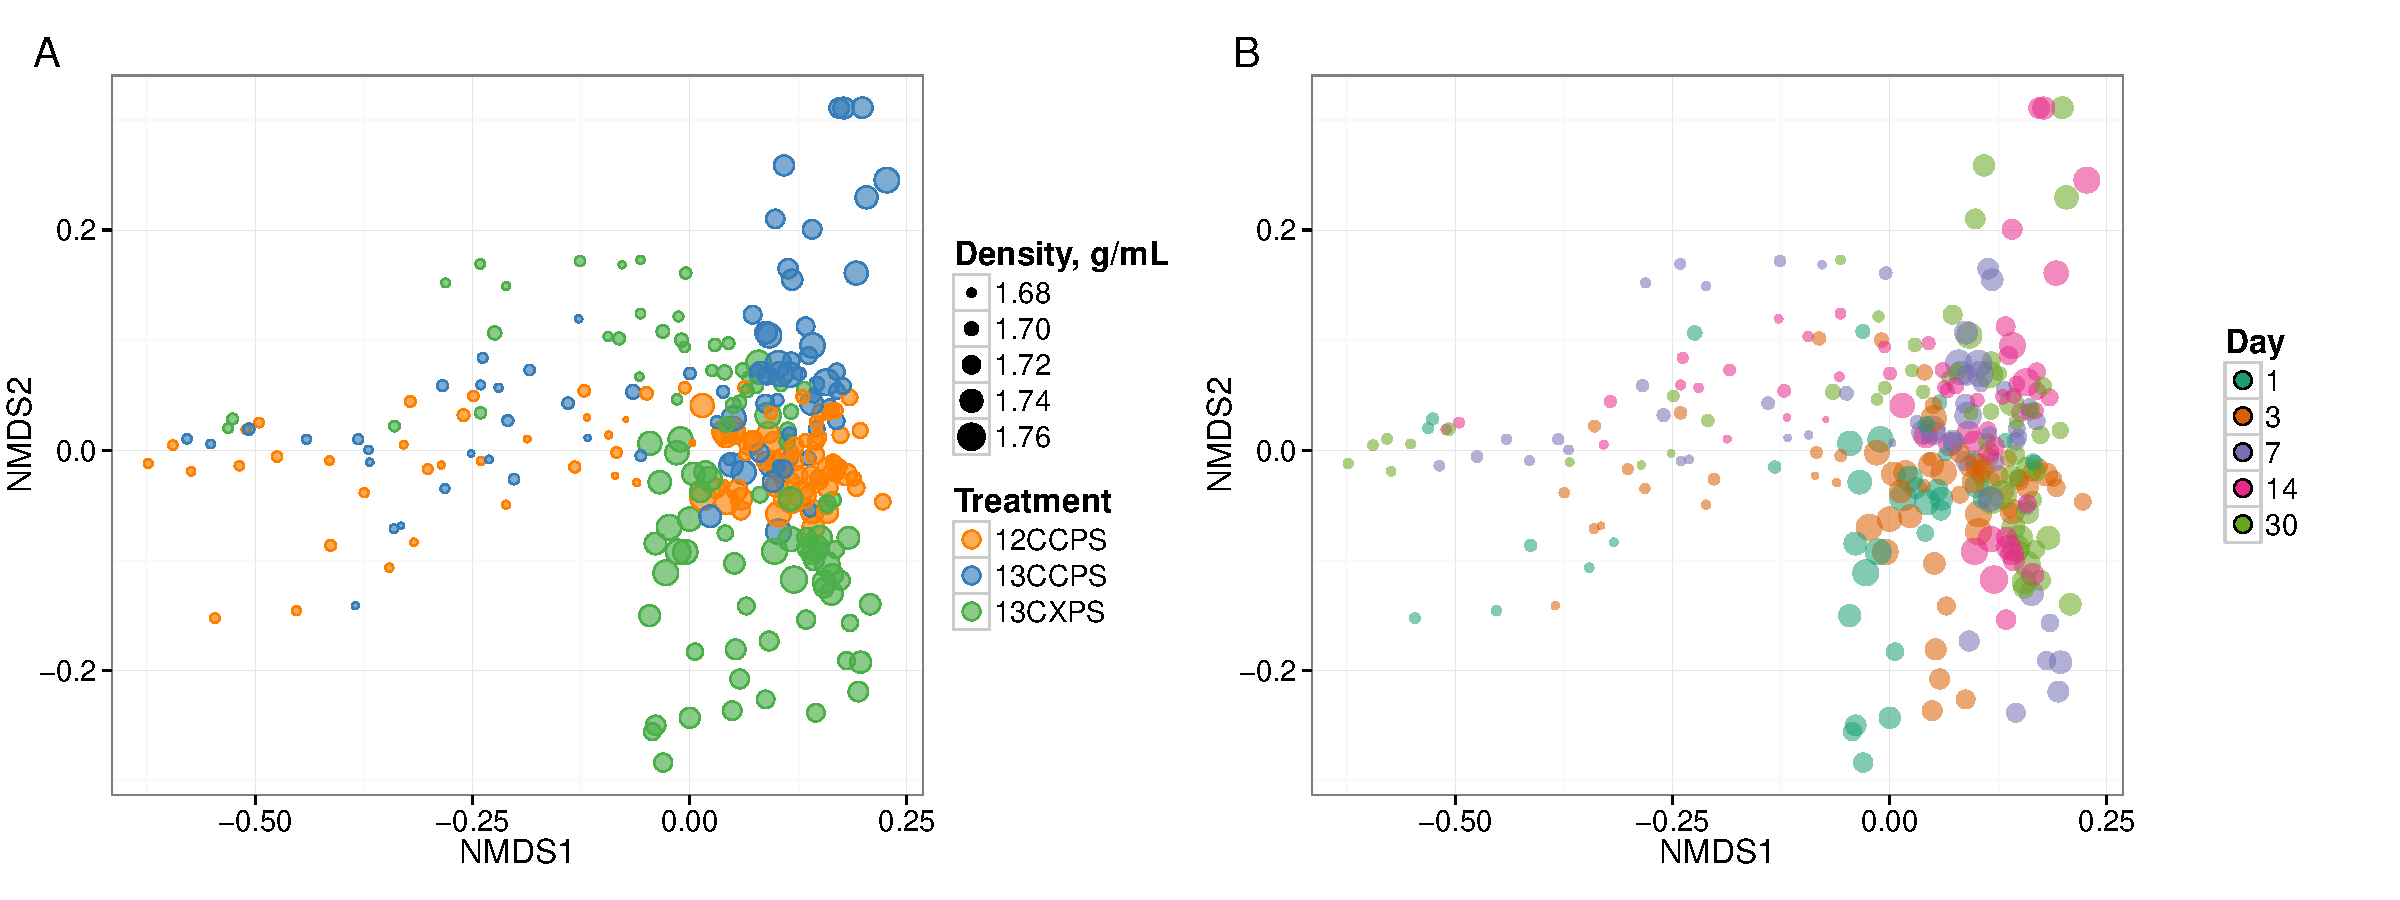
\includegraphics[width=15.4cm]{figures/ordination_all1/ordination_all.pdf}}
    \caption{\protectNMDS ordination of SSU rRNA gene sequence composition in
gradient fractions shows that it is
a function of many factors including fraction density, isotopic labeling, and
time. Dissimilarity in SSU rRNA gene sequence composition was quantified using the 
weighted UniFrac metric. SSU rRNA gene sequencess were surveyed in twenty
gradient fractions at each sampling point for each treatment (Figure~S1).
$^{13}$C-labeling of DNA is apparent because the SSU rRNA gene sequence composition of
gradient fractions from $^{13}$C and control treatments differ at high density.
Each point on the NMDS plot represents one gradient fraction.  SSU rRNA gene sequence
composition differences between gradient fractions were quantified by the
weighted Unifrac metric. The size of each point is positively correlated with
density and colors indicate the treatment (A) or day (B).
}\label{fig:ord}
\end{center} \end{figure*}


\begin{figure*}[H]
	\begin{center}
	\centerline{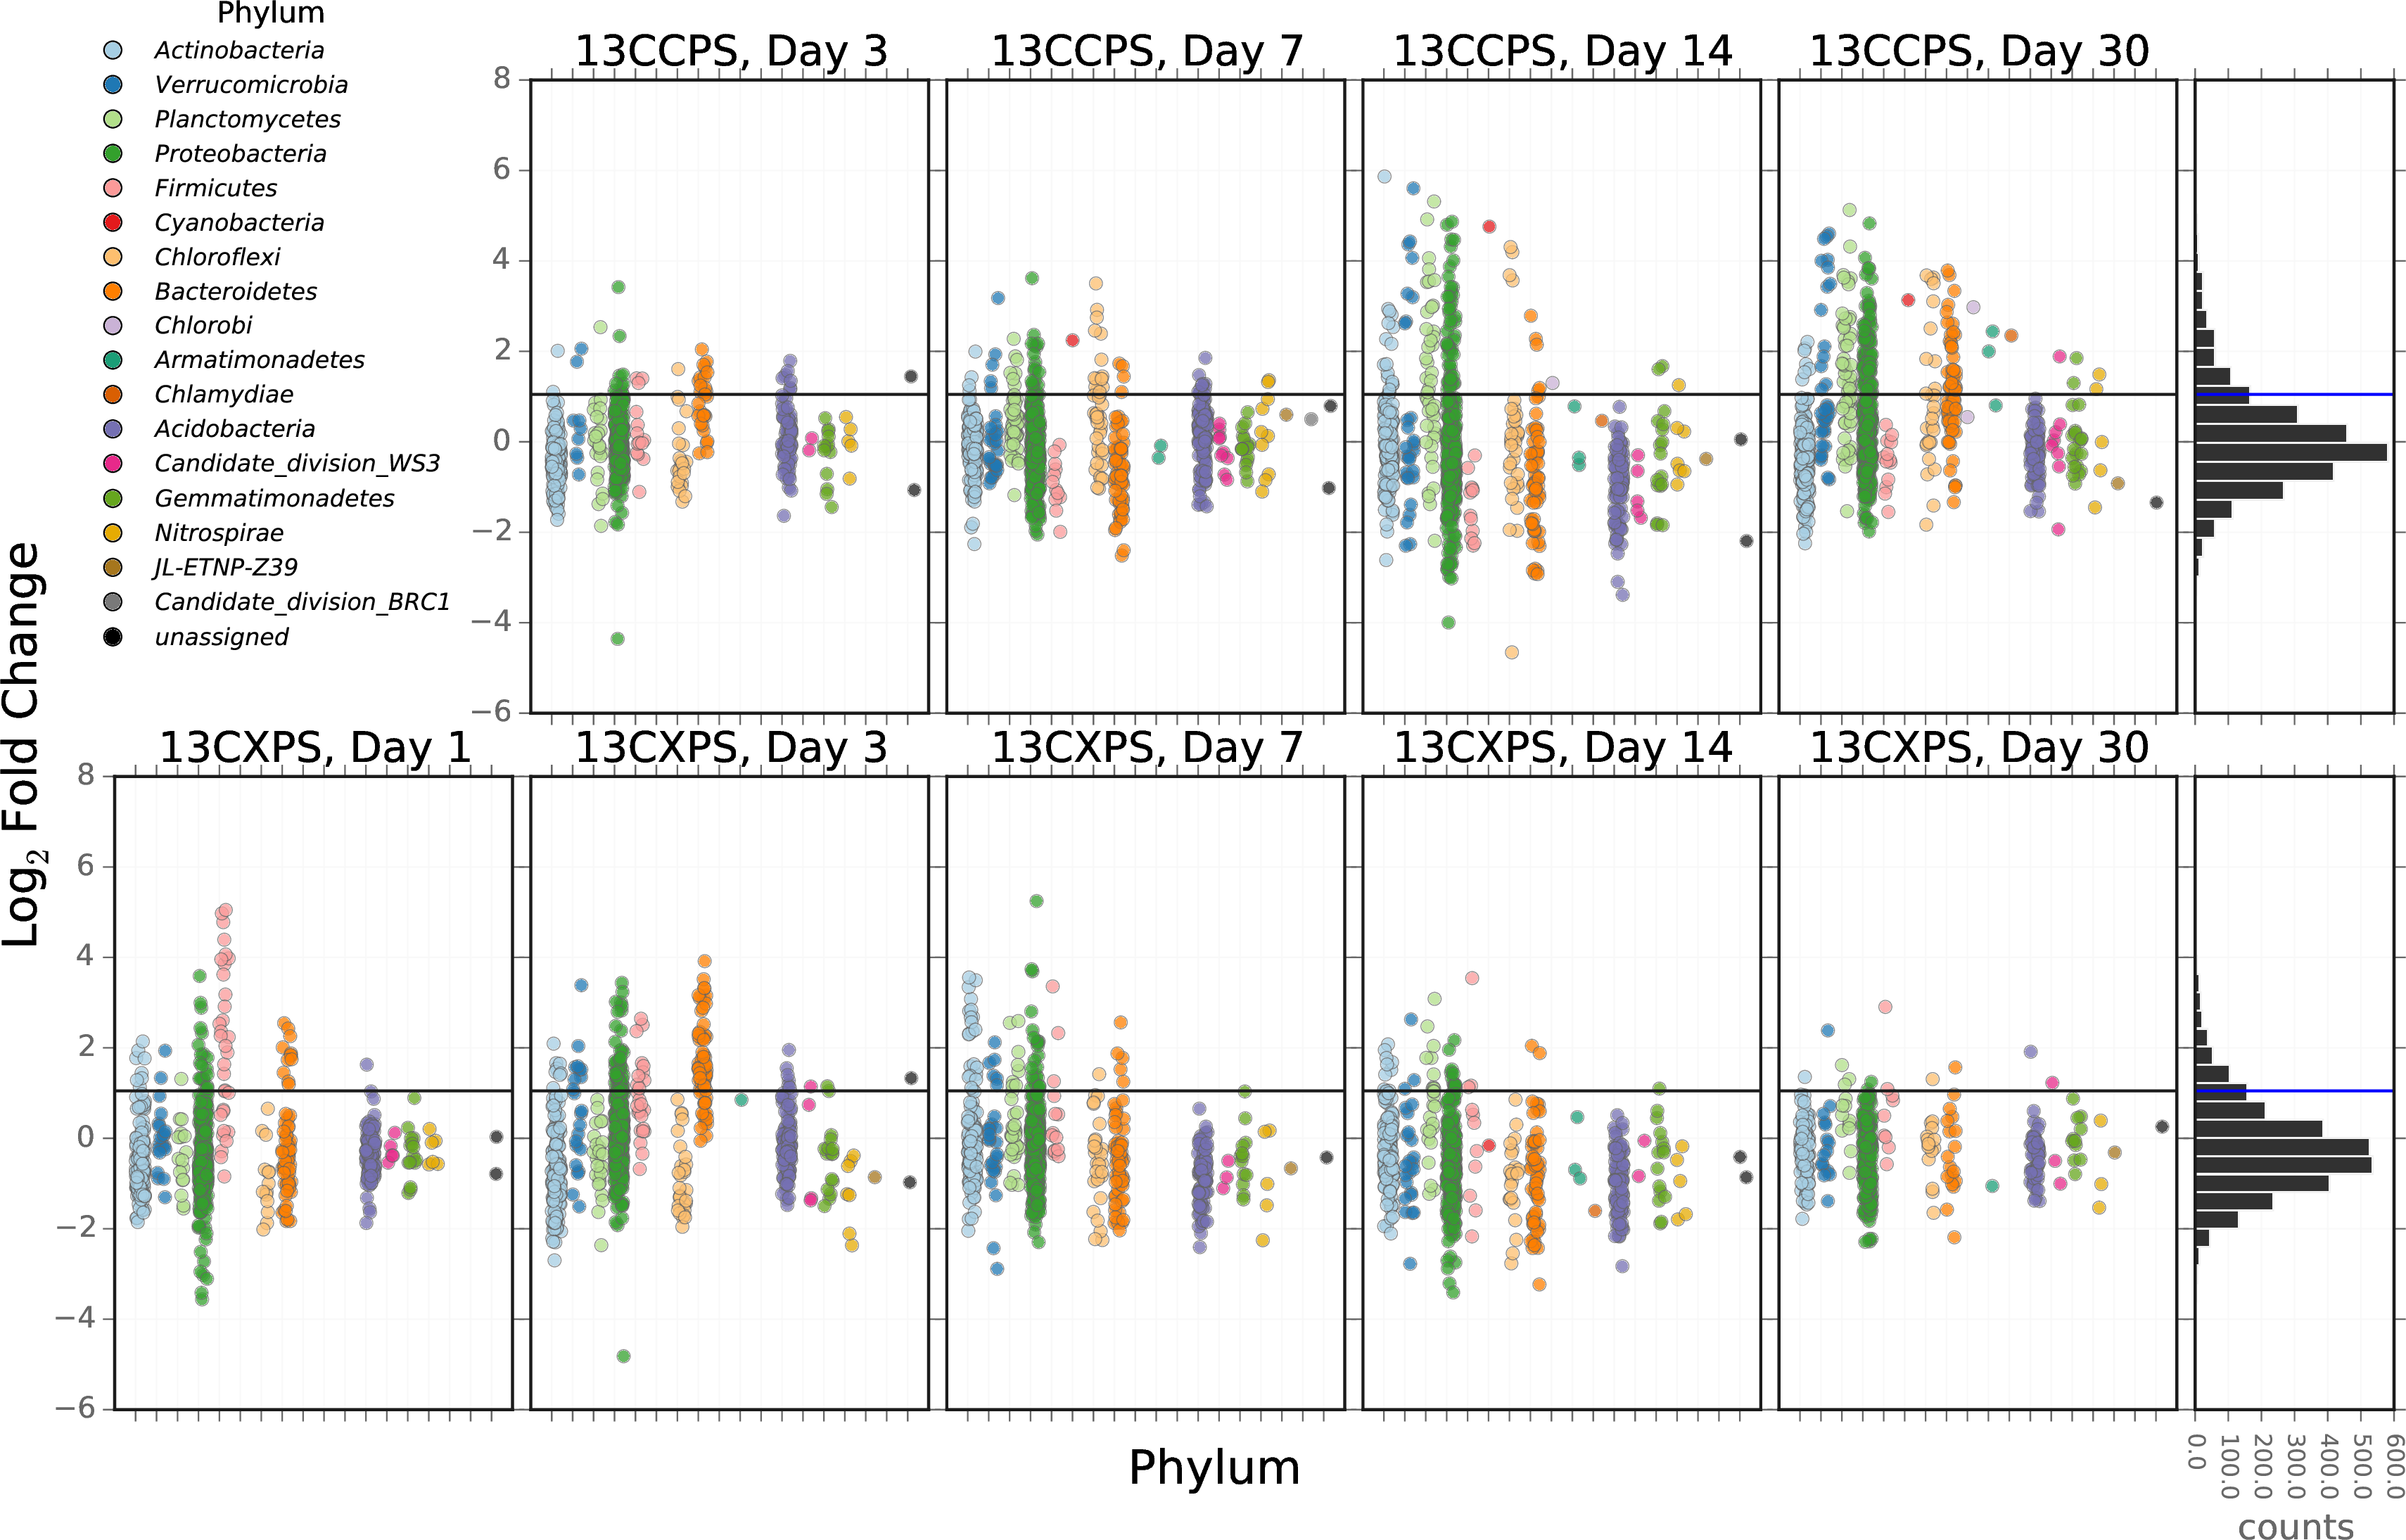
\includegraphics[width=15.4cm]{figures/l2fc_fig1/l2fc_fig.png}}
	\caption{\protectOTU enrichment in $^{13}$C-treatment heavy density fractions relative to control 
represented as LFC (see Methods) for the $^{13}$C-cellulose treatment (top) and
$^{13}$C-xylose treatment (bottom). High LFC indicate the OTU incorporated $^{13}$C into
DNA (each point represents an OTU-treatment-day combination). Different colors
represent different phyla and different panels represent different days. The
final column shows the frequency distribution of LFC values in each row.
Within each panel, shaded areas are used to indicate LFC plus or minus
one standard deviation (dark shading) or two standard devations (light shading) 
about the mean of all LFC values.
    
    
}\label{fig:l2fc}
        \end{center}
\end{figure*}

\begin{figure*}[H]
	\begin{center}
    \centerline{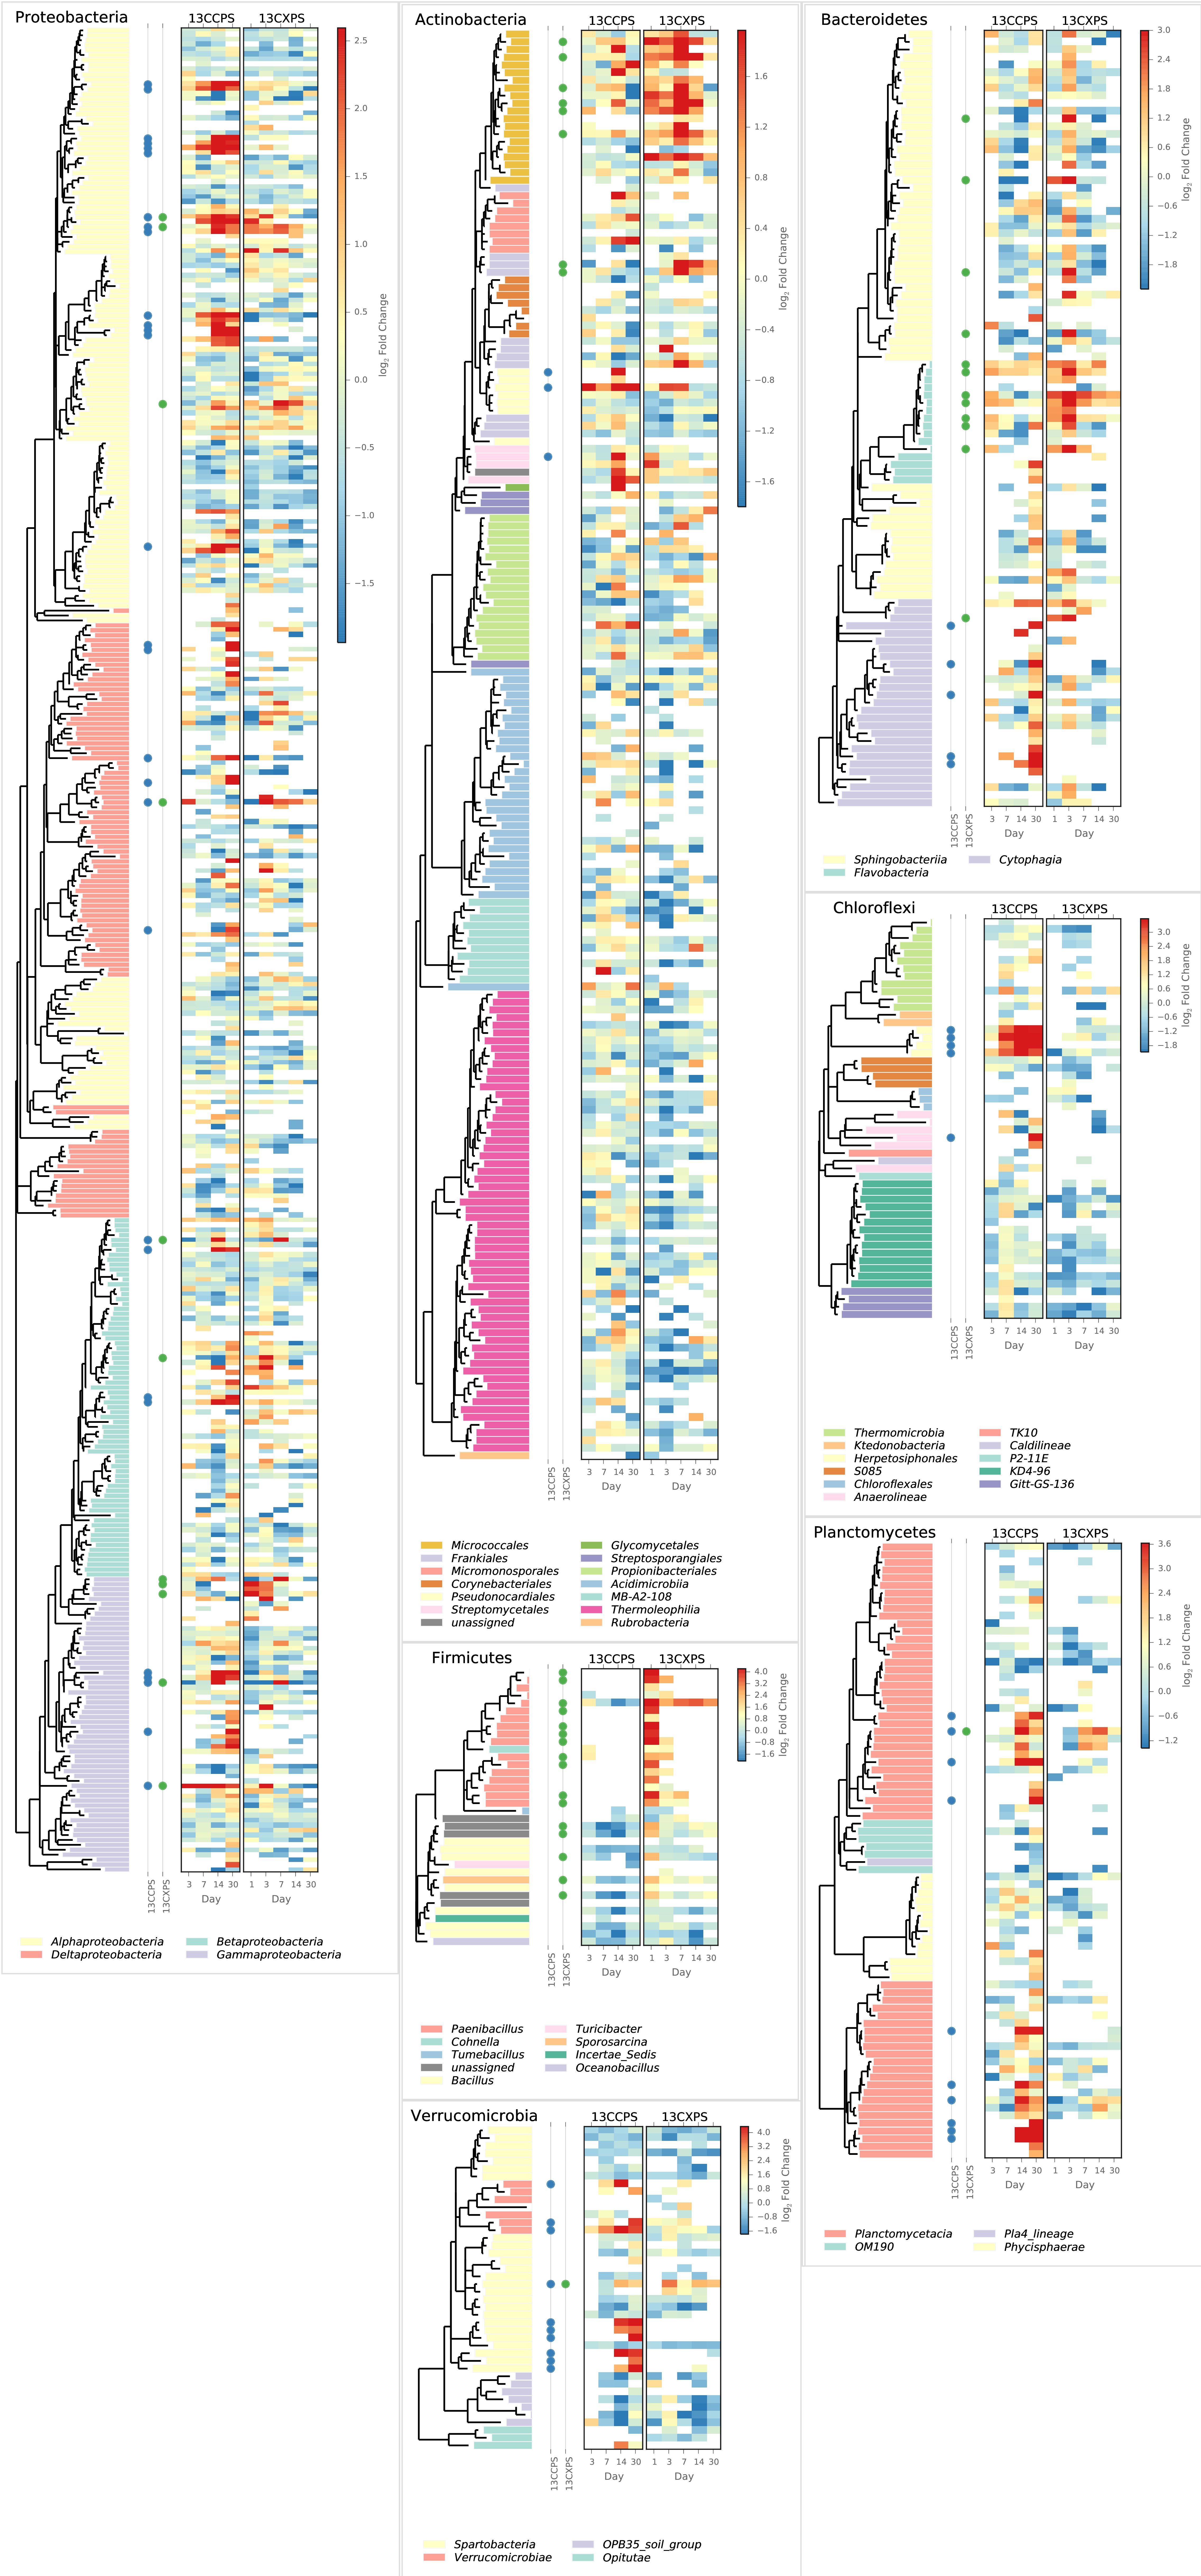
\includegraphics[width=0.65\textwidth]{figures/tiled_tree/tiled_tree.png}}
    \caption[Phylogenetic trees]{\protectPhylogenetic position of cellulose responders and xylose responders in the context of all OTUs that passed 
sparsity independent filtering criteria (see Methods). Only those phyla that contain responders are shown.
Colored dots are used to identify xylose responders (green) and cellulse
responders (blue). The heatmaps indicate enrichment in high denstiy fractions
relative to control (represented as LFC) for each OTU in response to both
$^{13}$C-cellulose (13CCPS, leftmost heatmap) and $^{13}$C-xylose
(13CXPS, rightmost heatmap) with values for different days in each heatmap
column. High enrichment values (represented as LFC) provide evidence of $^{13}$C-labeled DNA.  

}\label{fig:tiledtree}
    \end{center} 
\end{figure*}

\begin{figure*}[H]
	\begin{center}
	\centerline{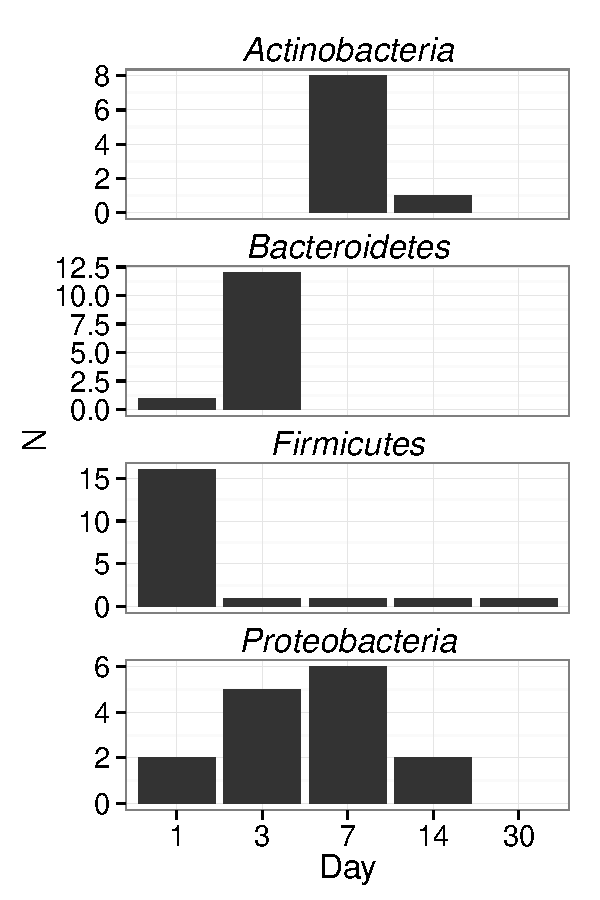
\includegraphics[width=0.6\textwidth]{figures/xylose_rspndr_bar/xylose_rspndr_bar.pdf}}
	\caption{\protectLeft column shows counts of $^{13}$C-xylose responders in the \textit{Actinobacteria, Bacteroidetes, Firmicutes} and \textit{Proteobacteria} at days 1, 3, 7 and 30. Right panel shows OTU fold enrichment in heavy gradient fractions for $^{13}$C-xylose amendment DNA relative to corresponding control fractions. 
    }\label{fig:xyl_count}
        \end{center}
\end{figure*}

\begin{figure*}[H]
	\begin{center}
	\centerline{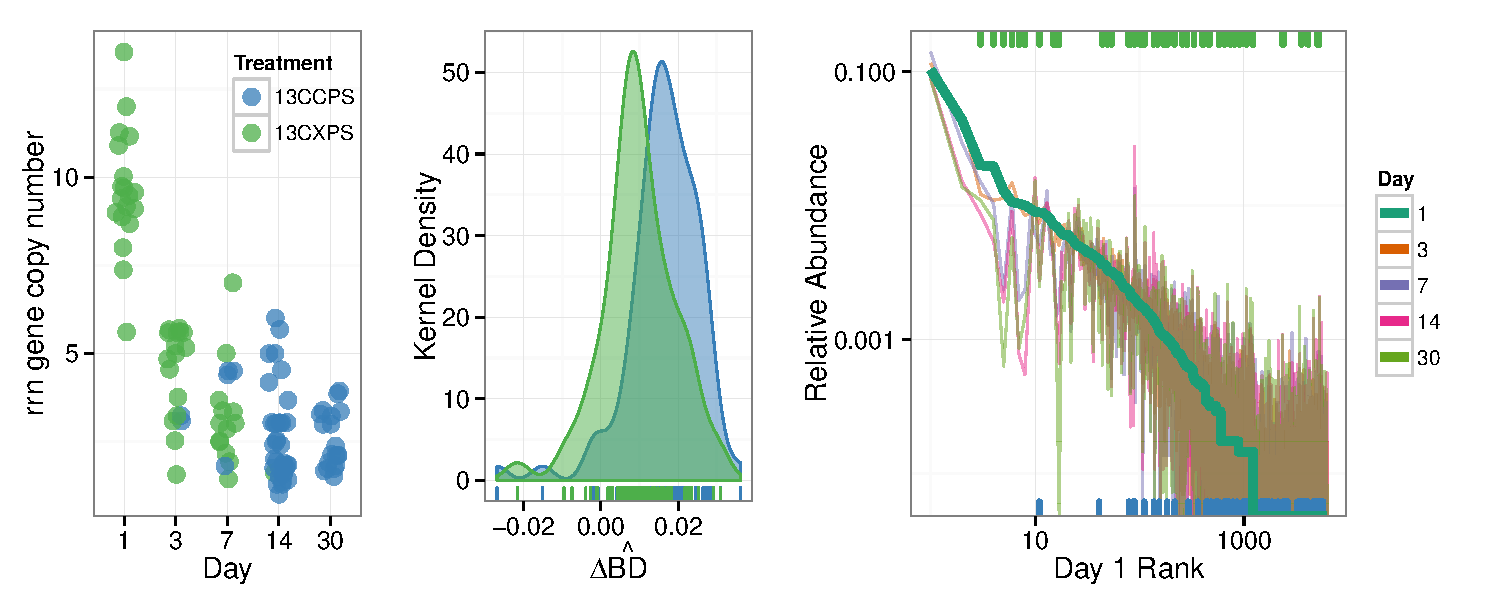
\includegraphics[width=15.4cm]{figures/shift_and_rabund3/shift_and_rabund.png}}
	\caption{\protectCharacteristics of xylose responders (green) and cellulose responders (blue)
based on estimated \textit{rrn} copy number (A), $\Delta\hat{BD}$ (B), and
relative abundance in non-fractionated DNA (C). The estimated \textit{rrn} copy
number of all responders is shown versus time (A). Kernel density histogram of
$\Delta\hat{BD}$ values shows cellulose responders had higher average
$\Delta\hat{BD}$ than xylose responders indicating higher average atom \%
$^{13}$C in OTU DNA (B). The final panel indicates the rank relative abundance
of all OTUs observed in the non-fractionated DNA (C) where rank was determined
at day 1 (bold line) and relative abundance for each OTU is indicated for all
days by colored lines (see legend). Xylose responders (green ticks) have higher
relative abundance in non-fractionated DNA than cellulose responders (green ticks). 
All ticks are based on day 1 relative abundance.
}\label{fig:shift}
    \end{center}
\end{figure*}


\restoregeometry
